%!TEX root = ../main.tex

\section{Постановка задачи}

\begin{frame}{Математическая модель}
\vspace{-0.3cm}
\begin{block}{Уравнения динамики системы}
	\begin{itemize}
		\item Уравнение электрического потенциала $\Phi$:
		\[
			\Div(\epsilon[\phi] \nabla \Phi) = 0
		\]
		\item Уравнение фазового поля $\phi$ (типа Аллена--Кана):
		\[
			\cfrac{1}{m} \partt{\phi} = \half \epsilon'(\phi) \gradsq{\Phi} + \cfrac{\Gamma}{l^2} f'(\phi) + \half \Gamma \Delta \phi
		\]
	\end{itemize}
\end{block}
\begin{itemize}
	\item Плотность свободной энергии
	\vspace{-0.2cm}
	\[
		\pi = -\half \epsilon[\phi] \gradsq{\Phi} + \Gamma \cfrac{1 - f(\phi)}{l^2} + \cfrac{\Gamma}{4} \gradsq{\phi}
	\]
\end{itemize}
\vspace{-1.9cm}
{\raggedleft Подробнее: \cite{ponomarev_stability}, \cite{zipunova_higher_codimension} \par}
\vspace{0.9cm}
\begin{columns}
\column{0.33\textwidth}
	\vspace{0.35cm}
	\[
		f(\phi) = 4 \phi^3 - 3 \phi^4
	\]
\column{0.33\textwidth}
	\[
		\epsilon(\vx, t) = \cfrac{\epsilon_0(\vx)}{f(\phi(\vx, t)) + \delta}
	\]
\column{0.33\textwidth}
\end{columns}
\end{frame}


\begin{frame}{Математическая модель}
\vspace{-0.3cm}
\begin{block}{Уравнения динамики системы}
	\begin{itemize}
		\item Уравнение электрического потенциала $\Phi$:
		\[
			\Div(\epsilon[\phi] \nabla \Phi) = 0
		\]
		\item Уравнение фазового поля $\phi$ (типа Аллена--Кана):
		\[
			\cfrac{1}{m} \partt{\phi} = -F'(\phi; |\nabla \Phi|) + \half \Gamma \Delta \phi
		\]
	\end{itemize}
\end{block}
\begin{itemize}
	\item Плотность свободной энергии
	\vspace{-0.2cm}
	\[
		\pi = F(\phi; |\nabla \Phi|) + \cfrac{\Gamma}{4} \gradsq{\phi}
	\]
	\item $m$, $\Gamma$ -- параметры модели, константы
\end{itemize}
\end{frame}


\begin{frame}{Разностная схема}
\vspace{-0.9cm}
\[
	\cfrac{1}{m} \partt{\phi} = -F'(\phi; |\nabla \Phi|) + \half \Gamma \partxx{\phi}
\]
\vspace{-0.4cm}
\begin{itemize}
	\item $|\nabla \Phi|$ -- параметр
\end{itemize}
\begin{block}{Разностная задача}
	\[
		\cfrac{1}{m} \cfrac{\phi_i^{j + 1} - \phi_i^j}{\tau} = -F'(\phi_i^j; |\nabla \Phi|) + \cfrac{\Gamma}{2} \cfrac{\phi_{i + 1}^j - 2 \phi_i^j + \phi_{i - 1}^j}{h^2}
	\]
	\[\phi_i^0 = \phi_0(ih); \quad \phi_0^j = \phi_l(j \tau); \quad \phi_n^j = \phi_r(j \tau)\]
	Сетка регулярная; $\tau$ -- шаг по времени, $h$ -- шаг по пространству.
\end{block}
Явная разностная схема первого порядка по времени, второго по пространству.
\end{frame}


\begin{frame}{Типичное решение}
\vspace{-0.4cm}
\begin{columns}
\column{0.88\textwidth}
\begin{figure}
	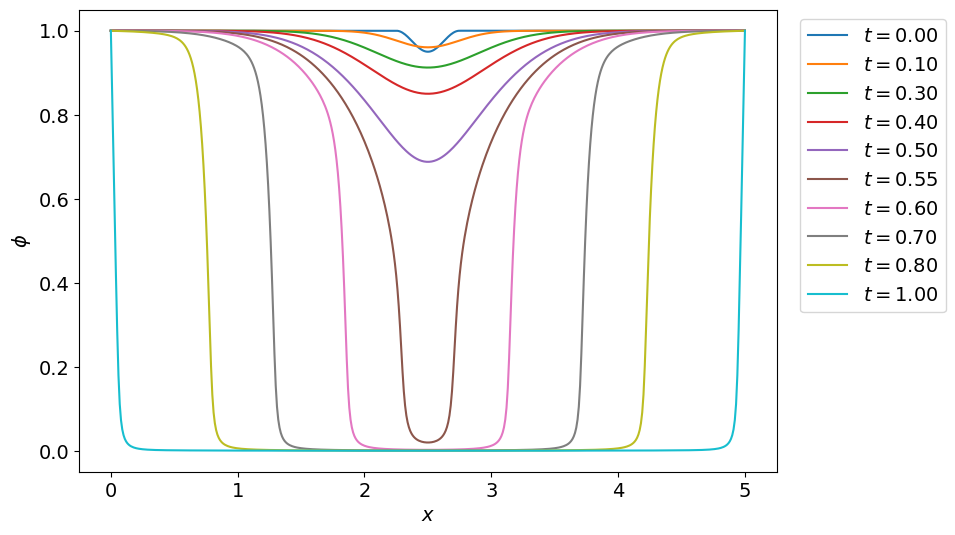
\includegraphics[width=\textwidth]{figures/typical_solution.png}
\end{figure}
\column{0.12\textwidth}
\hfill \\
\vspace{3.5cm}
\hspace{-2.5cm}
Из работы \cite{ponomarev_stability}. \\
\hspace{-2.5cm}
Узлов по измерениям: \\
\hspace{-2.5cm}
$N_x = 10^3$, $N_t = 10^5$
\end{columns}
\end{frame}


\begin{frame}{Цель работы}
\begin{itemize}
	\item Типичное поведение модели: долгий период медленных изменений, \\ затем стремительное развитие пробоя.
\end{itemize}
\begin{block}{Цель работы}
	Исследовать несколько подходов к адаптации расчетного шага по времени.
\end{block}
\end{frame}